% Options for packages loaded elsewhere
\PassOptionsToPackage{unicode}{hyperref}
\PassOptionsToPackage{hyphens}{url}
%
\documentclass[
  14,
  ignorenonframetext,
  aspectratio=141,
]{beamer}
\usepackage{pgfpages}
\setbeamertemplate{caption}[numbered]
\setbeamertemplate{caption label separator}{: }
\setbeamercolor{caption name}{fg=normal text.fg}
\beamertemplatenavigationsymbolsempty
% Prevent slide breaks in the middle of a paragraph
\widowpenalties 1 10000
\raggedbottom
\usepackage{amsmath,amssymb}
\usepackage{iftex}
\ifPDFTeX
  \usepackage[T1]{fontenc}
  \usepackage[utf8]{inputenc}
  \usepackage{textcomp} % provide euro and other symbols
\else % if luatex or xetex
  \usepackage{unicode-math} % this also loads fontspec
  \defaultfontfeatures{Scale=MatchLowercase}
  \defaultfontfeatures[\rmfamily]{Ligatures=TeX,Scale=1}
\fi
\usepackage{lmodern}
\usetheme[]{CambridgeUS}
\usecolortheme{dolphin}
\usefonttheme{structurebold}
\ifPDFTeX\else
  % xetex/luatex font selection
\fi
% Use upquote if available, for straight quotes in verbatim environments
\IfFileExists{upquote.sty}{\usepackage{upquote}}{}
\IfFileExists{microtype.sty}{% use microtype if available
  \usepackage[]{microtype}
  \UseMicrotypeSet[protrusion]{basicmath} % disable protrusion for tt fonts
}{}
\makeatletter
\@ifundefined{KOMAClassName}{% if non-KOMA class
  \IfFileExists{parskip.sty}{%
    \usepackage{parskip}
  }{% else
    \setlength{\parindent}{0pt}
    \setlength{\parskip}{6pt plus 2pt minus 1pt}}
}{% if KOMA class
  \KOMAoptions{parskip=half}}
\makeatother
\usepackage{xcolor}
\newif\ifbibliography
\usepackage{graphicx}
\makeatletter
\def\maxwidth{\ifdim\Gin@nat@width>\linewidth\linewidth\else\Gin@nat@width\fi}
\def\maxheight{\ifdim\Gin@nat@height>\textheight\textheight\else\Gin@nat@height\fi}
\makeatother
% Scale images if necessary, so that they will not overflow the page
% margins by default, and it is still possible to overwrite the defaults
% using explicit options in \includegraphics[width, height, ...]{}
\setkeys{Gin}{width=\maxwidth,height=\maxheight,keepaspectratio}
% Set default figure placement to htbp
\makeatletter
\def\fps@figure{htbp}
\makeatother
\setlength{\emergencystretch}{3em} % prevent overfull lines
\providecommand{\tightlist}{%
  \setlength{\itemsep}{0pt}\setlength{\parskip}{0pt}}
\setcounter{secnumdepth}{-\maxdimen} % remove section numbering
\newlength{\cslhangindent}
\setlength{\cslhangindent}{1.5em}
\newlength{\csllabelwidth}
\setlength{\csllabelwidth}{3em}
\newlength{\cslentryspacingunit} % times entry-spacing
\setlength{\cslentryspacingunit}{\parskip}
\newenvironment{CSLReferences}[2] % #1 hanging-ident, #2 entry spacing
 {% don't indent paragraphs
  \setlength{\parindent}{0pt}
  % turn on hanging indent if param 1 is 1
  \ifodd #1
  \let\oldpar\par
  \def\par{\hangindent=\cslhangindent\oldpar}
  \fi
  % set entry spacing
  \setlength{\parskip}{#2\cslentryspacingunit}
 }%
 {}
\usepackage{calc}
\newcommand{\CSLBlock}[1]{#1\hfill\break}
\newcommand{\CSLLeftMargin}[1]{\parbox[t]{\csllabelwidth}{#1}}
\newcommand{\CSLRightInline}[1]{\parbox[t]{\linewidth - \csllabelwidth}{#1}\break}
\newcommand{\CSLIndent}[1]{\hspace{\cslhangindent}#1}
\usepackage{booktabs,caption}
\usepackage[flushleft]{threeparttable}
\usepackage{tabularx}
\usepackage{amsfonts}
\usepackage{amsmath}
\usepackage{amssymb}


\ifLuaTeX
  \usepackage{selnolig}  % disable illegal ligatures
\fi
\IfFileExists{bookmark.sty}{\usepackage{bookmark}}{\usepackage{hyperref}}
\IfFileExists{xurl.sty}{\usepackage{xurl}}{} % add URL line breaks if available
\urlstyle{same}
\hypersetup{
  pdftitle={The impact of Basel III implementation on bank lending in South Africa},
  pdfauthor={Xolani Sibande and Alistair Milne},
  hidelinks,
  pdfcreator={LaTeX via pandoc}}

\title{The impact of Basel III implementation on bank lending in South
Africa}
\author{Xolani Sibande and Alistair Milne}
\date{5 December 2023}
\institute{South African Reserve Bank and Loughborough University}

\begin{document}
\frame{\titlepage}

\begin{frame}{Introduction}
\protect\hypertarget{introduction}{}
\begin{itemize}
\tightlist
\item
  This paper investigates the impact of the higher regulatory capital
  requirements of the implementation of the Basel III in South Africa
  between 2013 and 2019.
\item
  The principal data employed is monthly balance sheet data
\item
  Focus on a small set of large banks has some advantages: business
  models of these banks are similar
\item
  Our empirical specification follows previous studies of the impact of
  capital requirements on bank credit supply (for UK Aiyar \emph{et al.}
  (2014); for Peru Fang \emph{et al.} (2020))
\item
  We find little evidence of the impact of Basel III on lending
\end{itemize}
\end{frame}

\begin{frame}{Incremental implementation of capital requirments}
\protect\hypertarget{incremental-implementation-of-capital-requirments}{}
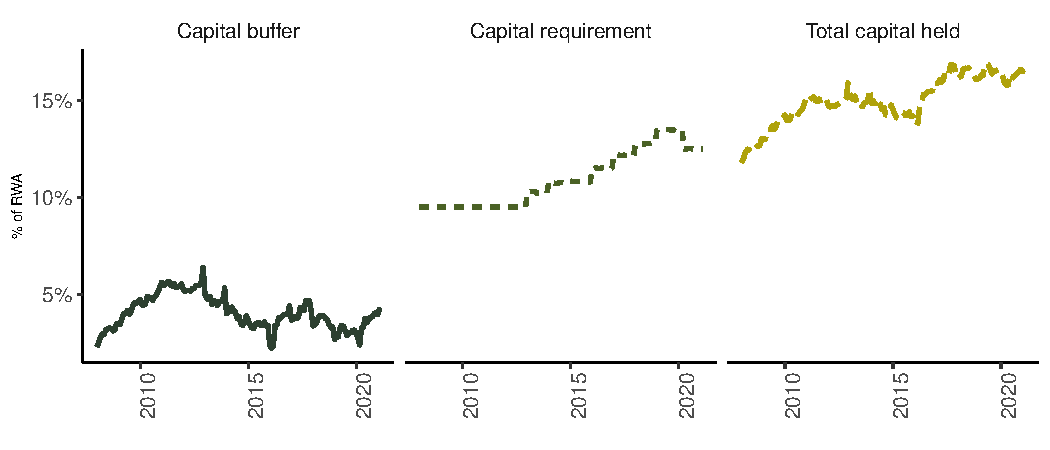
\includegraphics{baseIII_and_bank_lending_files/figure-beamer/capital-1.pdf}
\end{frame}

\begin{frame}{Data}
\protect\hypertarget{data}{}
\begin{itemize}
\tightlist
\item
  We collected data on the four major South African banks: Absa Bank,
  Standard Bank, First National Bank, and Nedbank
\item
  Mainly utilised the BA900s (bank economic returns) and the BA930s
  (bank product lending rates)
\item
  The Basel III capital requirements (BA700s) data was collected from
  the Prudential Authority
\item
  From the Prudential Authority, we also collected the controls data
\item
  We focus on real economic activity lending in the BA900s is
  represented by lending to households and non-financial corporations.
\item
  However, the BA900s only report granular lending categories to
  households and non-financial corporations. Therefore, some aggregation
  was necessary.
\item
  This aggregation essentially limited our sample to the big four
  lenders
\item
  Three major categories for households and non financial corporations
  (secured, unsecured, and mortgages)
\end{itemize}
\end{frame}

\begin{frame}{Methodology}
\protect\hypertarget{methodology}{}
Building on Fang \emph{et al.} (2020):

\(\Delta LOAN^i_{t, t-s} = \beta \Delta KR^i_{t, t-1} + \lambda \Delta KS^i_{t, t-1} + \alpha \Delta Demand^i_{t, t-1} + \gamma' \pmb{X}^i_{t-s} + \phi^i + \tau_t + \varepsilon^i_t.\)

\begin{itemize}
\tightlist
\item
  \(^i\) refers to the four banks
\item
  \(\Delta LOAN^i_{t, t-s}\) is the log difference of lending
\item
  \(\Delta KR^i_{t, t-1}\) is the change in the minimum capital
  requirement
\item
  \(\Delta Demand^i_{t, t-1}\) is the lending demand proxy represented
\item
  \(\pmb{X}^i_{t-s}\) is a bank level controls set at month \(t-s\).
\item
  The fixed effects (\(\phi^i\)) estimate other unobserved differences
  in bank characteristics.
\item
  To account for other factors, such as changes in the macroeconomic
  environment, we employ time-fixed effects (\(\tau_t\)).
\item
  \(\varepsilon^i_t\) using bank clustered standard errors
\end{itemize}
\end{frame}

\begin{frame}{Results Household Secured Credit (Example)}
\protect\hypertarget{results-household-secured-credit-example}{}
\begin{table}
\centering\begingroup\fontsize{10}{12}\selectfont

\resizebox{\linewidth}{!}{
\begin{tabular}{>{\raggedright\arraybackslash}p{7cm}lllll}
\toprule
\multicolumn{6}{c}{Household secured credit} \\
\cmidrule(l{3pt}r{3pt}){1-6}
  & (1) & (2) & (3) & (4) & (5)\\
\midrule
$\Delta KR_{t,t-1}$ & -0.1185 & -0.1941 & -0.3583 & 0.3135 & 0.0831\\
 & (0.1152) & (0.2621) & (0.2719) & (0.3298) & (0.3021)\\
$\Delta KS_{t,t-1}$ &  & -0.0815 & -0.0355 & -0.0102 & 0.0281\\
 &  & (0.1587) & (0.1773) & (0.1248) & (0.1390)\\
$\Delta Demand_{t,t-1}$ &  &  & 0.0032 &  & 0.0031\\
\addlinespace
 &  &  & (0.0042) &  & (0.0052)\\
$ROA_{t-1}$ &  &  &  & 0.2672 & 0.1810\\
 &  &  &  & (1.3378) & (1.3242)\\
$ROE_{t-1}$ &  &  &  & -0.0900 & -0.0816\\
 &  &  &  & (0.1107) & (0.1170)\\
\addlinespace
$Liquidity_{t-1}$ &  &  &  & -0.0081 & -0.0076\\
 &  &  &  & (0.0068) & (0.0085)\\
Num.Obs. & 372 & 372 & 369 & 368 & 365\\
Test of equality (p-value) & 0.35 & 0.65 & 0.18 & 0.11 & 0.95\\
Adj.R squared & 0.28 & 0.28 & 0.28 & 0.31 & 0.31\\
\bottomrule
\multicolumn{6}{l}{\rule{0pt}{1em}\textit{Note: }}\\
\multicolumn{6}{l}{\rule{0pt}{1em}The dependant variables in loan growth at bank level at a monthly frequency, calculated as the log difference at t and t -1.}\\
\multicolumn{6}{l}{\rule{0pt}{1em}Standard errors are clustered at a bank level.}\\
\multicolumn{6}{l}{\rule{0pt}{1em}All equations include both bank and monthly effects. A test for equality p-value of < 0.1 is significant.}\\
\multicolumn{6}{l}{\rule{0pt}{1em}*** p < 0.01, ** p < 0.05, * p < 0.1)}\\
\end{tabular}}
\endgroup{}
\end{table}
\end{frame}

\begin{frame}{Conclusion}
\protect\hypertarget{conclusion}{}
\begin{itemize}
\tightlist
\item
  While our set up is similar to Fang et al.~(2020), we find very much
  weaker evidence of an impact of capital requirements on the supply of
  bank lending.
\item
  We investigate the impact three categories of lending for both
  household and corporate borrowers.
\item
  Only in the case of secured credit for non-financial corporations do
  we obtain a statistically significant and economically sensible
  coefficient estimates and the coefficient is relatively small.
\item
  Exploring alternative dynamic estimation similarly yields little
  evidence of any.
\end{itemize}
\end{frame}

\begin{frame}{References}
\protect\hypertarget{references}{}
\hypertarget{refs}{}
\begin{CSLReferences}{0}{0}
\leavevmode\vadjust pre{\hypertarget{ref-aiyar2014international}{}}%
Aiyar, S., Calomiris, C. W., Hooley, J., Korniyenko, Y. and Wieladek, T.
(2014). {`The international transmission of bank capital requirements:
Evidence from the UK'}. \emph{Journal of Financial Economics}. Elsevier,
113 (3), pp. 368--382.

\leavevmode\vadjust pre{\hypertarget{ref-fang2020bank}{}}%
Fang, X., Jutrsa, D., Peria, S. M., Presbitero, A. F. and Ratnovski, L.
(2020). {`Bank capital requirements and lending in emerging markets: The
role of bank characteristics and economic conditions'}. \emph{Journal of
Banking \& Finance}. Elsevier, p. 105806.

\end{CSLReferences}
\end{frame}

\end{document}
